
\chapter{太阳}
\section{太阳内部}
\begin{figure}[hbt]
  \centering
  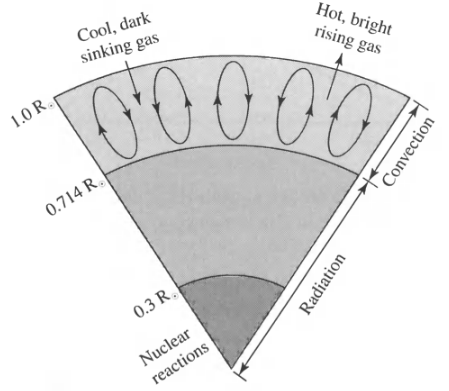
\includegraphics[width=9cm]{chapters/11/interior}
  \caption{太阳内部示意图。太阳内部可大致分为最中心的核反应区、中间的辐射区、最外层的对流区}
  \label{}
\end{figure}

\section{太阳大气}
\begin{figure}[hbt]
  \centering
  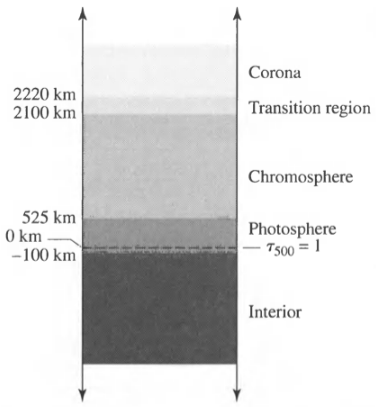
\includegraphics[width=6cm]{chapters/11/atmosphere}
  \caption{太阳大气示意图}
  \label{}
\end{figure}

\subsection{光球层}
光球层是太阳连续谱主要产生的区域,而上方的大气又会在连续谱上产生吸收线,这些吸收线最早由夫琅和费发现,因此被命名为\textbf{夫琅和费线}。

其中$\tau_{500}=1$被定义为\textbf{恒星表面},往下100\,km为光球层底部,往上温度降低,到525km高度降到最低4400\,K,这里被定义为光球层顶部。

观测上能看到恒星表面有明显的被称为\textbf{米粒组织}的对流区域,如图\ref{fig:cell},亮暗是温度不同造成的,亮的区域是高温气体上升到表面,向周围扩散冷却后下沉,对应边缘较暗的区域。

\begin{figure}[hbt]
  \centering
  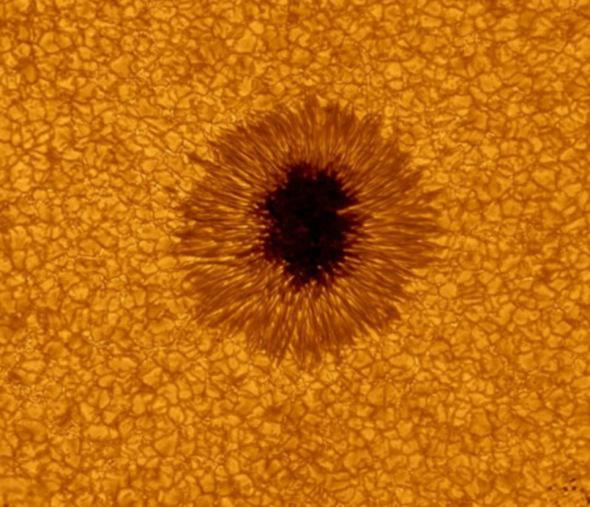
\includegraphics[width=6cm]{chapters/11/cell}
  \caption{米粒组织和太阳黑子}
  \label{fig:cell}
\end{figure}

由于恒星是由气体组成,不像地球这样的固体行星是刚体转动,在任何地方都有相同的自转角速度,恒星在不同纬度和不同深度处的气体自转角速度并不相同,如图\ref{fig:rotaion}所示,太阳维度越高的区域,自转角速度越小,而在内部辐射区以内,极高的密度,使这里的转动接近刚体,具有相同的转速。

\begin{figure}[hbt]
  \centering
  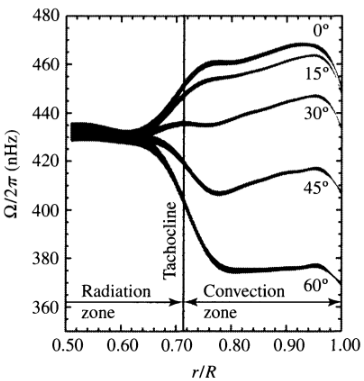
\includegraphics[width=6cm]{chapters/11/rotation}
  \caption{太阳的自选频率随深度和纬度的分布}
  \label{fig:rotaion}
\end{figure}



\subsection{色球层}
光球层之上,太阳表面上方2100\,km以下的范围,是一个很强的谱线产生区域,很多在低温高密度的光球层无法产生的谱线会在这里被产生。

\subsection{过渡区}
位于色球层以上,底部的100\,km,温度从4400\,K上升到$10^5$\,K,变化非常快;后面部分平缓增加到$10^6$\,K,在过渡区的不同高度能够观测到电磁波谱的紫外和极紫外部分。

\subsection{日冕层}
色球层以上,密度和光度都非常低的高温电离区,只有在日食的时候才能够看到日冕,日冕由于密度极低,不适合看作局部热平衡,因此也不适合定义准确温度。观测到的日冕结构可以主要分成以下三部分:
\begin{itemize}
  \item K冕,取自德语的``连续"(\textit{Kontinuierlich}),因为自由电子散射了来自光球层的可见光而被看见
  \item F冕,取自夫琅和费,因为尘埃反射了夫琅和费线而被看见
  \item E冕,由于电离气体的发射线而被看见
\end{itemize}

观测上显示,日冕发出的光并不是均匀的,有的区域比较亮,有的区域比较暗,较暗的区域被称为\textbf{日冕空洞}。这种现象的形成是由于太阳的磁场分布导致的,太阳的磁场近似是偶极磁场,由于磁场线能够束缚等离子体,磁场强的区域会导致比较亮(粒子的辐射)。而在一些磁场``开放''区域,磁场线能够延伸到距离太阳很远的区域,离子也会顺着这样的磁场线逃向远方,这也就形成了\textbf{太阳风}。

高温等离子体中的磁场通常会被``冻结'',从而跟随着等离子体运动,而在在受到一些垂直于磁场方向的扰动时,也会有相应的回复力,同时产生横波——\textbf{阿尔文波}。

\section{太阳周期}
\paragraph{太阳黑子}
如图\ref{fig:cell}黑色部分为太阳黑子,是磁场很强的区域,太阳表面的黑子数量变化会有11年的周期,在此期间,黑子的数量会不断增加,并且向赤道方向靠近。

\paragraph{太阳耀斑}
一种能量释放的过程,其产生机制是由于\textbf{磁重连},相反方向的磁场线靠得较近时,会断裂然后连接形成新的磁场线,在这个过程中会导致原本绕着磁场线旋转的离子被大量抛出。

\paragraph{日珥}
色球层中的一种大型结构,其形成也是与磁场相关

\paragraph{日冕物质抛射}
被认为也是由大型的磁重连事件导致的大量日冕物质被抛出。

\paragraph{太阳磁场}
太阳的磁场近似偶极磁场,同时也具有和太阳黑子一样,每隔11年会倒转N-S极方向,因此目前认为这种现象和太阳黑子的运动有关。由于太阳的较差自转,赤道处的气体比两极快,由于磁冻结效应,赤道处的磁场也会跟着较快自转,这就会导致一段时间后磁场会极度扭曲,发生磁重连。
